\documentclass{beamer}
\usetheme[sectionpage=progressbar, subsectionpage=progressbar, numbering=fraction, progressbar=foot, block=fill, background=light]{metropolis}
\usepackage{appendixnumberbeamer}
\usepackage{textpos}
\usepackage{booktabs}
\usepackage[scale=2]{ccicons}

\usepackage{pgfplots}
\usepgfplotslibrary{dateplot}
\usetikzlibrary{backgrounds}
\usepackage{xspace}
\newcommand{\themename}{\textbf{\textsc{metropolis}}\xspace}
\title{Attention based models in End-to-End ASR}
\subtitle{Exploration of Attention in ESPNET toolkit}
\date{\today}
\author{Shreekantha Nadig}
\institute{International Institute of Information Technology - Bangalore}
%\titlegraphic{\hfill\includegraphics[height=1.5cm]{logo.pdf}}

\usepackage{tikz}
\usetikzlibrary{shapes,shadows,arrows,patterns, matrix}

\tikzstyle{line} = [draw, -latex']
\tikzstyle{round} = [draw, circle, fill=black!30, minimum size=4em, node distance=4em, font=\fontsize{30}{10}\selectfont]
\tikzstyle{mlp_enc} = [rectangle, draw, fill=red!50, text width=2cm, minimum height=5em, text centered, node distance=10em, font=\fontsize{20}{10}\selectfont]
\tikzstyle{mlp_att} = [rectangle, draw, fill=green!50, text width=2cm, minimum height=5em, text centered, node distance=10em, font=\fontsize{20}{10}\selectfont]
\tikzstyle{mlp_dec} = [rectangle, draw, fill=blue!50, text width=2cm, minimum height=5em, text centered, node distance=10em, font=\fontsize{20}{10}\selectfont]
\tikzstyle{enc_h} = [rectangle, draw,  pattern=horizontal lines, pattern color=red!60, text width=1cm, minimum height=10em, minimum width=3em, text centered, node distance=10em, font=\fontsize{25}{10}\selectfont]
\tikzstyle{atts} = [rectangle, draw,  pattern=horizontal lines, pattern color=green!70, text width=1cm, minimum height=10em, minimum width=3em, text centered, node distance=10em, font=\fontsize{20}{10}\selectfont]
\tikzstyle{dec_z} = [rectangle, draw,  pattern=horizontal lines, pattern color=blue!60, text width=1cm, minimum height=10em, minimum width=3em, text centered, node distance=10em, font=\fontsize{20}{10}\selectfont]
\tikzstyle{cnn} = [rectangle, draw,  pattern=crosshatch, pattern color=red!50!blue!50, text width=2cm, minimum height=5em, text centered, node distance=10em, font=\fontsize{20}{10}\selectfont]
\tikzstyle{box} = [rectangle, draw,  fill=blue!20, text width=3cm, minimum height=5em, minimum width=3em, text centered, node distance=10em, font=\fontsize{20}{10}\selectfont]

\begin{document}
	\addtobeamertemplate{frametitle}{}{%
		\begin{textblock*}{100mm}(.97\textwidth,-1cm)
			{
\includegraphics[width=2.5em]{iiitb_logo.png}}
		\end{textblock*}}

\maketitle

\begin{frame}{Table of contents}
	\setbeamertemplate{section in toc}[sections numbered]
	\tableofcontents[hideallsubsections]
\end{frame}



\section{Introduction}

\begin{frame}[fragile]{2D Location Aware Attention}
\begin{center}
	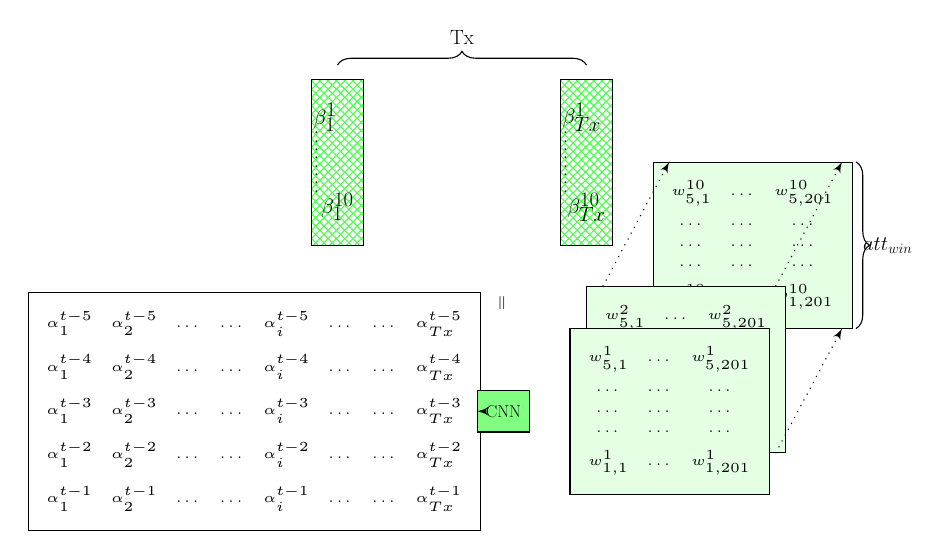
\begin{tikzpicture}[scale=0.3, every node/.style={transform shape, font=\fontsize{5}{10}\selectfont}]
	\matrix [matrix of nodes, draw, .style={nodes={draw=none, minimum width=1em}}] (m)
	{
		$\alpha_{1}^{t-5}$ & $\alpha_{2}^{t-5}$ & \dots  & \dots & $\alpha_{i}^{t-5}$ & \dots & \dots & $\alpha_{Tx}^{t-5}$ \\
		
		$\alpha_{1}^{t-4}$ & $\alpha_{2}^{t-4}$ & \dots  & \dots & $\alpha_{i}^{t-4}$ & \dots & \dots & $\alpha_{Tx}^{t-4}$ \\
		
		$\alpha_{1}^{t-3}$ & $\alpha_{2}^{t-3}$ & \dots  & \dots & $\alpha_{i}^{t-3}$ & \dots & \dots & $\alpha_{Tx}^{t-3}$ \\
		
		$\alpha_{1}^{t-2}$ & $\alpha_{2}^{t-2}$ & \dots  & \dots & $\alpha_{i}^{t-2}$ & \dots & \dots & $\alpha_{Tx}^{t-2}$ \\
		
		$\alpha_{1}^{t-1}$ & $\alpha_{2}^{t-1}$ & \dots  & \dots & $\alpha_{i}^{t-1}$ & \dots & \dots & $\alpha_{Tx}^{t-1}$ \\
	};

	\node [mlp_att, right of=m, node distance = 30em] (cnn1) {CNN};
	\path [line] (m.east) to (cnn1.west);
	\matrix [matrix of nodes, right of = cnn1,fill=green!10, node distance = 20em, draw, .style={nodes={draw=none, minimum width=1em}}] (m1)
	{
		$w_{5,1}^{1}$ & \dots & $w_{5,201}^{1}$ \\
		
		\dots & \dots & \dots \\
		
		\dots & \dots & \dots \\
		
		\dots & \dots & \dots \\
		
		$w_{1,1}^{1}$ & \dots & $w_{1,201}^{1}$ \\
	};
	
	\begin{scope}[on background layer]
	\matrix [matrix of nodes, above of = m1, fill=green!10, xshift=10em, node distance = 20em, draw, .style={nodes={draw=none, minimum width=1em}}] (m3)
	{
		$w_{5,1}^{10}$ & \dots & $w_{5,201}^{10}$ \\
		
		\dots & \dots & \dots \\
		
		\dots & \dots & \dots \\
		
		\dots & \dots & \dots \\
		
		$w_{1,1}^{10}$ & \dots & $w_{1,201}^{10}$ \\
	};
	\end{scope}
	
	\begin{scope}[on background layer]
		\matrix [matrix of nodes, above of = m1, fill=green!10, xshift=2em, node distance = 5em, draw, .style={nodes={draw=none, minimum width=1em}}] (m2)
		{
			$w_{5,1}^{2}$ & \dots & $w_{5,201}^{2}$ \\
			
			\dots & \dots & \dots \\
			
			\dots & \dots & \dots \\
			
			\dots & \dots & \dots \\
			
			$w_{1,1}^{2}$ & \dots & $w_{1,201}^{2}$ \\
		};
	\end{scope}
	
	
	\draw [decorate,decoration={brace,amplitude=5pt, raise=0.5em}] (m3.43) -- (m3.-43) node [black,midway, xshift=5.5em] {\fontsize{25}{10}\selectfont $att_{win}$};
	
	\path [line, dotted] (m2.135) to (m3.135);
	\path [line, dotted] (m2.43) to (m3.43);
	\path [line, dotted] (m2.-43) to (m3.-43);
	
	\node [atts, above of = cnn1, pattern=crosshatch, node distance = 30em, minimum height = 20em, text width=2cm,font=\fontsize{40}{10}\selectfont, xshift=-20em] (b1) {$\beta_{1}^{1}$ \newline . \newline . \newline . \newline . \newline . \newline . \newline . \newline . \newline $\beta_{1}^{10}$} ;
	
	\node [atts, right of = b1, pattern=crosshatch, node distance = 30em, minimum height = 20em, text width=2cm,font=\fontsize{40}{10}\selectfont] (b2) {$\beta_{Tx}^{1}$ \newline . \newline . \newline . \newline . \newline . \newline . \newline . \newline . \newline $\beta_{Tx}^{10}$} ;
	
	\draw [decorate,decoration={brace,amplitude=5pt, raise=0.5em}] (b1.north) -- (b2.north) node [black,midway, yshift=5em] {\fontsize{40}{10}\selectfont Tx};
	
	\node [above of = cnn1, yshift=10em, font=\fontsize{40}{10}\selectfont] (eq1) {\rotatebox{90}{$\,=$}};
	\end{tikzpicture}
\end{center}
\end{frame}


	\begin{frame}[fragile]{2D Location Aware Attention - Full picture}
	\begin{center}
		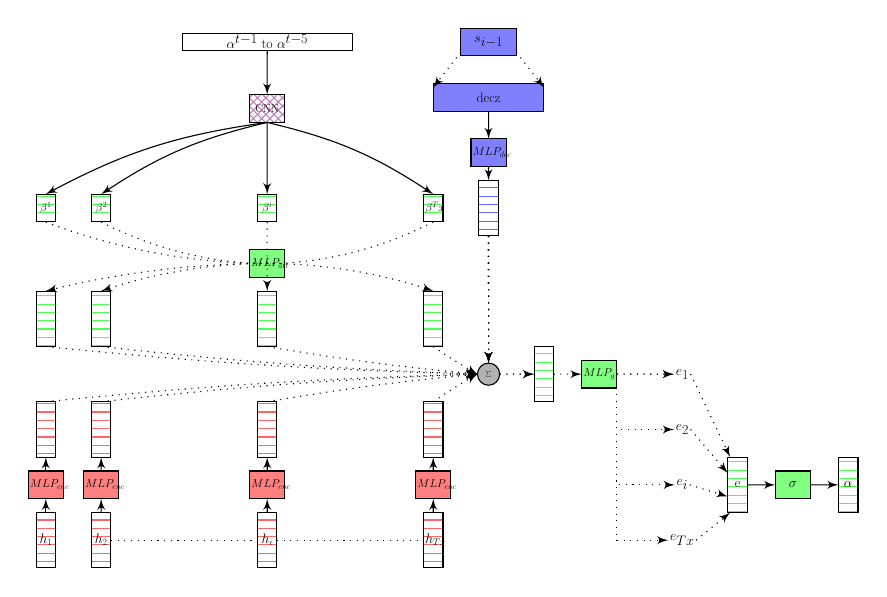
\begin{tikzpicture}[scale=0.2, every node/.style={transform shape}]
		\node [enc_h] (h1) {$h_{1}$};
		\node [enc_h,right of = h1] (h2) {$h_{2}$};
		\node [enc_h,right of = h2, node distance = 30em] (hi) {$h_{i}$};
		\node [enc_h,right of = hi, node distance = 30em] (hTx) {$h_{Tx}$};
		\draw [dotted] (h2.east) to (hi.west);
		\draw [dotted] (hi.east) to (hTx.west);
		
		
		\node [mlp_enc, above of = h1, node distance = 10em] (mlp1) {$MLP_{enc}$};
		\path [line] (h1.north) to (mlp1.south);
		\node [enc_h, above of = mlp1] (he1) {};
		\path [line] (mlp1.north) to (he1.south);
		
		
		\node [mlp_enc, above of = h2, node distance = 10em] (mlp2) {$MLP_{enc}$};
		\path [line] (h2.north) to (mlp2.south);
		\node [enc_h, above of = mlp2] (he2) {};
		\path [line] (mlp2.north) to (he2.south);
		
		
		\node [mlp_enc, above of = hi, node distance = 10em] (mlpi) {$MLP_{enc}$};
		\path [line] (hi.north) to (mlpi.south);
		\node [enc_h, above of = mlpi] (hei) {};
		\path [line] (mlpi.north) to (hei.south);
		
		
		\node [mlp_enc, above of = hTx, node distance = 10em] (mlpTx) {$MLP_{enc}$};
		\path [line] (hTx.north) to (mlpTx.south);
		\node [enc_h, above of = mlpTx] (heTx) {};
		\path [line] (mlpTx.north) to (heTx.south);
		
		\node [draw, rectangle, above of=hei, node distance = 70em,font=\fontsize{40}{10}\selectfont, text width = 30em, text centered] (alpha_t) {$\alpha^{t-1}$ to $\alpha^{t-5}$};
		
		\node [cnn, below of=alpha_t, node distance = 12em] (cnn1) {CNN};
		\path [line] (alpha_t.south) to (cnn1.north);
		\node [atts, above of = he1,minimum height=5em, node distance = 40em] (beta1) {$\beta^1$};
		\node [atts, above of = he2, minimum height=5em, node distance = 40em] (beta2) {$\beta^2$};
		\node [atts, above of = hei, minimum height=5em, node distance = 40em] (betai) {$\beta^i$};
		\node [atts, above of = heTx, minimum height=5em, node distance = 40em] (betaTx) {$\beta^Tx$};
		
		\path [line] (cnn1.south) to [bend right=10] (beta1.north);
		\path [line] (cnn1.south) to [bend right=10] (beta2.north);
		\path [line] (cnn1.south) to (betai.north);
		\path [line] (cnn1.south) to [bend left=10] (betaTx.north);
		
		\node [mlp_att, below of=betai, node distance = 10em] (mlpatt) {$MLP_{att}$};
		\node [atts, below of = beta1, node distance = 20em] (beta1_enc) {};
		\node [atts, below of = beta2, node distance = 20em] (beta2_enc) {};
		\node [atts, below of = betai, node distance = 20em] (betai_enc) {};
		\node [atts, below of = betaTx, node distance = 20em] (betaTx_enc) {};
		\path [line, dotted] (beta1.south) parabola bend (mlpatt) (beta1_enc.north);
		\path [line, dotted] (beta2.south) parabola bend (mlpatt) (beta2_enc.north);
		\path [line, dotted] (betai.south) parabola bend (mlpatt) (betai_enc.north);
		\path [line, dotted] (betaTx.south) parabola bend (mlpatt) (betaTx_enc.north);
		
		\node [round, below of=betaTx_enc, node distance=10em, xshift=10em] (sum1) {$\sum$};
		
		\node [mlp_dec, right of = betaTx, node distance = 10em, minimum width = 10em, yshift=30em, font=\fontsize{40}{10}\selectfont] (sim1) {$s_{i-1}$};
		\node [mlp_dec, below of=sim1, minimum width = 20em, font=\fontsize{40}{10}\selectfont] (dec_z) {decz};
		\path [line, dotted] (sim1.200) to (dec_z.170);
		\path [line, dotted] (sim1.-20) to (dec_z.10);
		\node [mlp_dec, below of=dec_z, node distance = 10em] (mlp_dec) {$MLP_{dec}$};
		\path [line] (dec_z) to (mlp_dec);
		\node [dec_z, below of = mlp_dec] (decz_enc) {};
		\path [line] (mlp_dec) to (decz_enc);

		\path [line, dotted] (beta1_enc.south) to [bend right=2] (sum1.west);
		\path [line, dotted] (he1.north) to [bend left=2] (sum1.west);
		\path [line, dotted] (decz_enc.south) to (sum1.north);
		
		\path [line, dotted] (beta2_enc.south) to [bend right=2] (sum1.west);
		\path [line, dotted] (he2.north) to [bend left=2] (sum1.west);
		\path [line, dotted] (decz_enc.south) to (sum1.north);
		
		\path [line, dotted] (betai_enc.south) to [bend right=2] (sum1.west);
		\path [line, dotted] (hei.north) to [bend left=2] (sum1.west);
		\path [line, dotted] (decz_enc.south) to (sum1.north);
		
		\path [line, dotted] (betaTx_enc.south) to [bend right=2] (sum1.west);
		\path [line, dotted] (heTx.north) to [bend left=2] (sum1.west);
		\path [line, dotted] (decz_enc.south) to (sum1.north);
		
		\node [atts, right of=sum1, node distance = 10em] (asdf) {};
		\node [mlp_att, right of=asdf] (mlpg) {$MLP_{g}$};
		\node [right of=mlpg, node distance=15em, font=\fontsize{40}{10}\selectfont] (e1) {$e_1$};
		
		\node [below of=e1, node distance=10em, font=\fontsize{40}{10}\selectfont] (e2) {$e_2$};
		
		\node [below of=e2, node distance=10em, font=\fontsize{40}{10}\selectfont] (ei) {$e_i$};
		
		\node [below of=ei, node distance=10em, font=\fontsize{40}{10}\selectfont] (eTx) {$e_{Tx}$};
		
		\node [atts, right of=ei, font=\fontsize{40}{10}\selectfont] (e) {e};
		
		\path [line, dotted] (e1.east) to (e.105);
		\path [line, dotted] (e2.east) to (e.130);
		\path [line, dotted] (ei.east) to (e.-130);
		\path [line, dotted] (eTx.east) to (e.-105);
		
		\node [mlp_att, right of=e, font=\fontsize{40}{10}\selectfont] (sm) {$\sigma$};
		\path [line] (e.east) to (sm.west);
		
		
		\node [atts, right of=sm, font=\fontsize{40}{10}\selectfont] (alphas) {$\alpha$};
		\path [line] (sm.east) to (alphas.west);
		
		\path [line, dotted] (sum1.east) to (asdf.west);
		\path [line, dotted] (sum1.east) to (asdf.west);
		\path [line, dotted] (asdf.east) to (mlpg.west);
		\path [line, dotted] (mlpg.east) to (e1.west);
		\path [line, dotted] (mlpg.east) to (e1.west);
		\path [line, dotted] (mlpg.east) |- (e2.west);
		\path [line, dotted] (mlpg.east) |- (ei.west);
		\path [line, dotted] (mlpg.east) |- (eTx.west);
		
		
		\end{tikzpicture}
	\end{center}
	\end{frame}
\end{document}